
This experiment regards only flux-tunable qubits since it studies the flux dependency of the resonator frequency.

As we saw in \cref{sec:flux_tunable_qubits}, for flux-tunable qubits there is a bias level, called \textit{sweetspot}, where the qubit frequency is almost non dependant from flux oscillations.
It is extremely important to find, at least roughly, this bias level before doing qubit spectroscopy (so before finding the qubit frequency) otherwise the qubit will have a completely different frequency than the one at normal working bias (we are talking of differences of hundreds of MHz or even GHz).

Because of that, we can proceed with a variant of a resonator spectroscopy experiment where we also change the bias~\cite{Greene2014}.
Note that the resonator is not directly affected by it, but it changes is resonance frequency in accordance to the qubit one that is directly dependent on the bias.

Since we are tying to exploit the coupling between qubit and resonator, we need to operate in the low power regime.

The experiment, repeated for a certain number of shots, for different frequencies and biases, will have the following layout:
\begin{itemize}
    \item we send a constant DC current at the qubit through the flux line. The voltage amplitude of this "pulse"\footnote{This can be done by connecting a constant source or, as in our case, sending a long constant and not modulated pulse.} will be the bias level;
    \item after waiting few nanoseconds to be sure that the qubit is stable, we can measure the resonator at the amplitude level found with the punchout experiment;
    \item we set again the bias a zero (this is extremely important because DC currents tend to heat up the cryostat).
\end{itemize}

We expect to see a parabola-like dependence as in \cref{fig:flux_resonator_spectroscopy_sketch}.
\begin{figure}[ht]
    \centering
    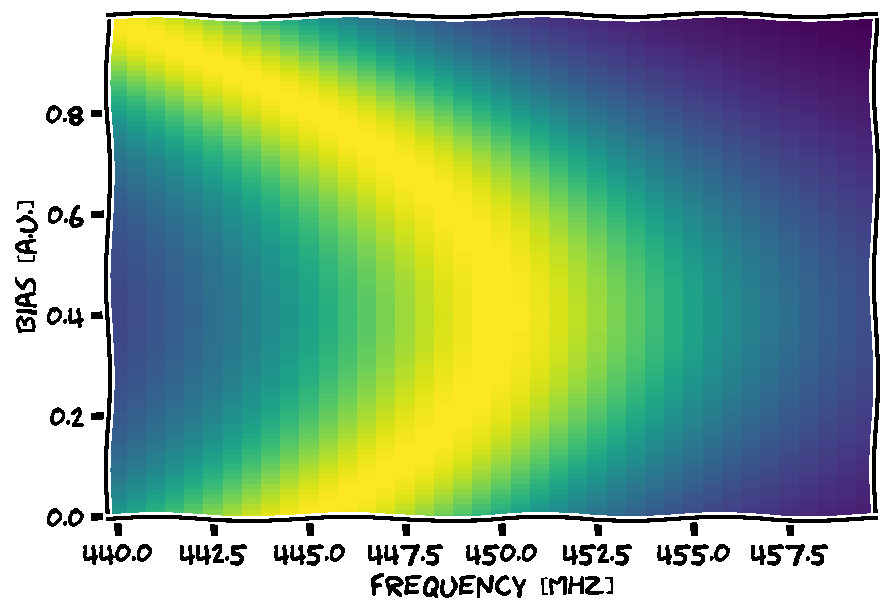
\includegraphics[width=8cm]{characterization/figures/resonator_spectroscopy_flux_sketch.pdf}
    \caption{Expected plot for a flux resonator spectroscopy experiment.}
    \label{fig:flux_resonator_spectroscopy_sketch}
\end{figure}
From this plot we can set the sweetspot level at $\approx 0.4$ [a.u.].
Note that we do not have a great resolution and we will later have to execute a similar experiment with the qubit resonance, that is much more dependent on the flux.

\noindent
A real plot is presented in \cref{fig:resonators_flux}.

Something that is also very important is to consider all the qubits at once (if there is more than one).
We need to set all qubits at their sweetspot even for experiments that do not concern them, because they influence and change the sweetspots of all the other qubits.
For example, if we measure qubit\_0 alone we could find a sweetspot of 0.5, but when we measure it at the same time of qubit\_1 (that has a non-zero sweespot), then the first sweetspot shifts to 0.2.

\begin{figure}[ht]
    \makebox[\textwidth][c]{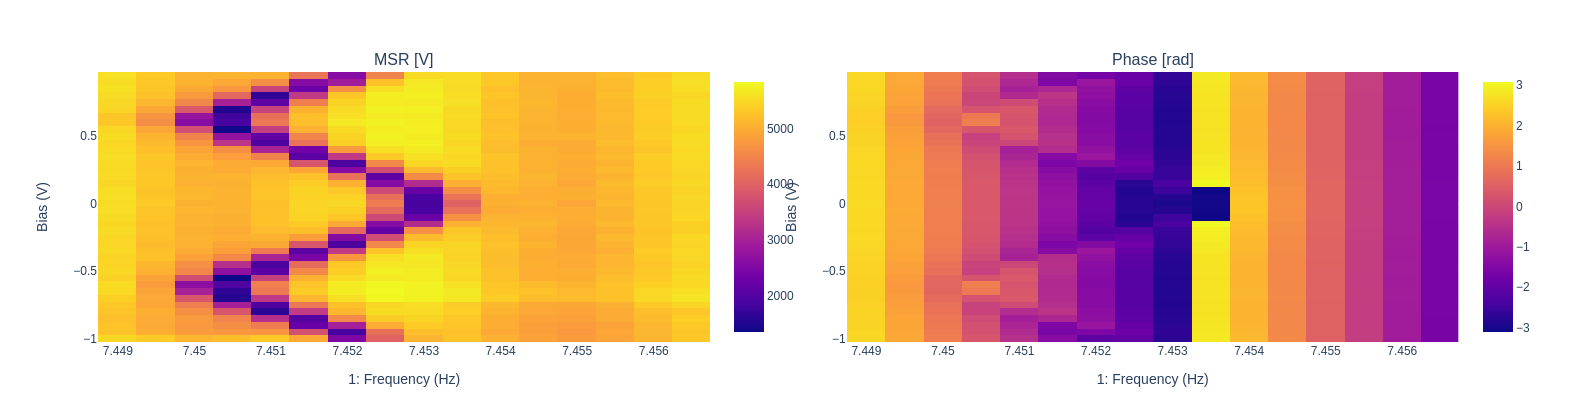
\includegraphics[width=1.3\textwidth]{characterization/figures/res_spec_flux.png}}
    \caption{Plot a the flux resonator spectroscopy experiment.}
    \label{fig:resonators_flux}
\end{figure}

\fluxexperimentrecap
{Flux resonator spectroscopy}
{readout calibration, flux dependence calibration}
{estimation of the flux sweetspot,\\resonator frequency at the sweetspot}
{a measurement is executed for different frequencies and different biases (fixing the amplitude). We do a 3D plot with transmitted signal vs frequency vs bias. We extract bias and frequency for the sweetspot (highest frequency)}
